\documentclass[a4paper, 10pt]{article}
\usepackage[cm]{fullpage}


\usepackage{listings}
\usepackage{color}

\definecolor{mygreen}{rgb}{0,0.6,0}
\definecolor{mygray}{rgb}{0.5,0.5,0.5}
\definecolor{mymauve}{rgb}{0.58,0,0.82}

\lstset{ %
  backgroundcolor=\color{white},   % choose the background color; you must add \usepackage{color} or \usepackage{xcolor}
  basicstyle=\footnotesize,        % the size of the fonts that are used for the code
  breakatwhitespace=false,         % sets if automatic breaks should only happen at whitespace
  breaklines=true,                 % sets automatic line breaking
  captionpos=b,                    % sets the caption-position to bottom
  commentstyle=\color{mygreen},    % comment style
  deletekeywords={...},            % if you want to delete keywords from the given language
  escapeinside={\%*}{*)},          % if you want to add LaTeX within your code
  extendedchars=true,              % lets you use non-ASCII characters; for 8-bits encodings only, does not work with UTF-8
  frame=single,                    % adds a frame around the code
  keepspaces=true,                 % keeps spaces in text, useful for keeping indentation of code (possibly needs columns=flexible)
  keywordstyle=\color{blue},       % keyword style
  language=Octave,                 % the language of the code
  morekeywords={*,...},            % if you want to add more keywords to the set
  numbers=left,                    % where to put the line-numbers; possible values are (none, left, right)
  numbersep=5pt,                   % how far the line-numbers are from the code
  numberstyle=\tiny\color{mygray}, % the style that is used for the line-numbers
  rulecolor=\color{black},         % if not set, the frame-color may be changed on line-breaks within not-black text (e.g. comments (green here))
  showspaces=false,                % show spaces everywhere adding particular underscores; it overrides 'showstringspaces'
  showstringspaces=false,          % underline spaces within strings only
  showtabs=false,                  % show tabs within strings adding particular underscores
  stepnumber=2,                    % the step between two line-numbers. If it's 1, each line will be numbered
  stringstyle=\color{mymauve},     % string literal style
  tabsize=2,                       % sets default tabsize to 2 spaces
  title=\lstname                   % show the filename of files included with \lstinputlisting; also try caption instead of title
}
\usepackage{graphicx} % Required for the inclusion of images
\usepackage{natbib} % Required to change bibliography style to APA
\usepackage{amsmath} % Required for some math elements 
\usepackage{soul}

\setlength\parindent{0pt} % Removes all indentation from paragraphs

\title{Seismic Processing \\ Prac 3 - Processing a real dataset.} % Title

\author{ERTH3021} % Author name

\date{\today} % Date for the report

\begin{document}

\maketitle % Insert the title, author and date
This is the last of three pracs on seismic data processing.  In this prac we will complete the processing of the synthetic dataset from prac2.   Once that is complete you will process a real dataset from scratch.
\par~\\
As with prac 1\& 2 code templates have been provided. The prac can be downloaded from  \\ \textbf{https://github.com/stuliveshere/Seismic-Processing-Prac3}

\section*{Introduction}
At the end of last week we created a seismic section from the foybrook model synthetic dataset. The resulting stack was of reasonable quality, considering the tools available.  However there are a number of processes missing which would normally be applied, including

\begin{itemize}
\item statics corrections
\item wavelet deconvolution
\item spatially variant velocity analysis
\item spectral windowing
\item spectral enhancement
\end{itemize}

Whilst statics corrections and wavelet deconvolution is outside the scope of this course, the remainder are not.
\par~\\
We are going to add 2 new processes to the work we did in prac 2. These processes are:

\begin{itemize}
\item spatially variant velocity analysis
\item spectral windowing
\end{itemize}

Once you have had some experience with these processes, you will process a real seismic dataset from (almost) scratch.

  
\subsection*{Exercise 1: Spatially Varying Velocity Analysis}
Why is performing velocity analysis on once CDP less than ideal? If the usual velocity analysis is performed every 100m (for shallow coal data) how many CDPS require velocity analysis?
\par~\\
Before we do velocity analysis/normal moveout correction we will need to initialise the dataset and perform a spherical divergence correction.  Once that is done select a range of CDPS to perform velocity anaysis on. 
\par~\\
The semblance analysis tool has been updated to make velocity anaysis easier. Use the new semblance tool to pick velocities for each CDP.
\par~\\
Build the velocity profile and display.  Make any changes neccessary to improve the consistency of the model. 
\par~\\
Stack the Foybrook model using the new velocity model.  Compare to the stack generated last week with a single velocity point.  Make note of any areas of improvement.

\subsection*{Exercise 2: Spectral Windowing}
A seismic dataset contains many signal frequencies.  Not all frequencies contain data.  For example very low frequencies and very high frequencies generally do not contain reflection information.  A frequency filter that cuts off low frequencies is referred to as a low-cut filter.  A frequency filter that cuts off high frequencies is referred to as a high-cut filter.  A frequency filter that cuts off both high and low is referred to as a bandpass filter.  
\par~\\
A fairly sophisticated bandpass filter has been added to the toolbox. A spectral analysis tool, called an FX filter, has also been added.  Load and display the stack from exercise 1 into the FX filter.  Discuss the resulting image and the possible location of the data.  Select a starting high and a low cut.
\par~\\
Apply the bandpass filter to the stack and compare to the stack with no filter.  Make the bandpass filter wider and narrower, comparing the result each time.  Select the best highcut and lowcut and apply to the data.  This section is referred to as the "final stack" for the foybrook model. Compare with the stack generated in prac 2. Highlight areas of improvement.

\section*{DIY Seismic Processing}
A dynamite survey has been supplied for you to process.  There are some pros and cons with processing dynamite.  Pros include high amplitude, high frequency signal.  Cons include cost.  Due to the cost, dynamite data is usually low fold.  This data also has some significant statics.  As such the data has been preprocessed to remove as much statics variation as possible.  Deconvolution has also been applied to the dataset.
\par~\\
Exercises 3 - 9 contain the templates required to process the supplied dataset, 'al\_dynamite.su'.  Each student is expected to hand in a processing report and email their final stack to uqsflet4@uq.edu.au.  The processing report should have the following format:
\par~\\
\begin{enumerate}
\item Introduction - one or two sentences explaining the data, including source type, source and reciever spacings, cdp spacings and fold.
\item Data Quality - discuss the data quality in a) shots, b) raw stack c) final stack d) spectral analysis
\item Processing
\begin{enumerate}
\item Initialisation - quick description, screenshot of representitive shot record
\item True Amplitude Recovery - describe TAR, screenshots of parameter testing (at least 3) and final parameter selected
\item Velocity Analysis - Screencapture and description of a representive semblance plot.  Discuss chosen CDP spacing.   Screencapture of final velocity field.
\item Stack - compare with stack generated with single velocity point. Highlight areas of improvement. Discuss other potential methods of velocity analysis. 
\item Bandpass Filter design - discuss the concept of spectral windowing.  Show screencapture of FX design window.  Discuss chosen highcut and lowcut thresholds.  Apply thresholds, and compare to stack with no bandpass filter. Highlight areas of improvement.  Vary the bandpass filter, and compare the results, with documentation.  Select best thresholds. 
\item Velocity Scaling - discuss the aim of velocity scaling.  Scale the velocities up and down and compare with the unscaled stack.  Highlight areas of improvement.  If neccessary, hand modify your velocity field.  Document and select best velocity field/scaling.
\item Trace Mix - discuss, test and apply pre-stack trace mix.   Compare to stack without trace mix and highlight areas of improvement.  Document testing and select best parameter.
\item Final stack - generate final stack.  include screencapture and table of key parameters.  email stack to uqsflet4@uq.edu.au (it should be around 1.7Mb).
\end{enumerate}
\end{enumerate}
\begin{figure}[h]
\centering
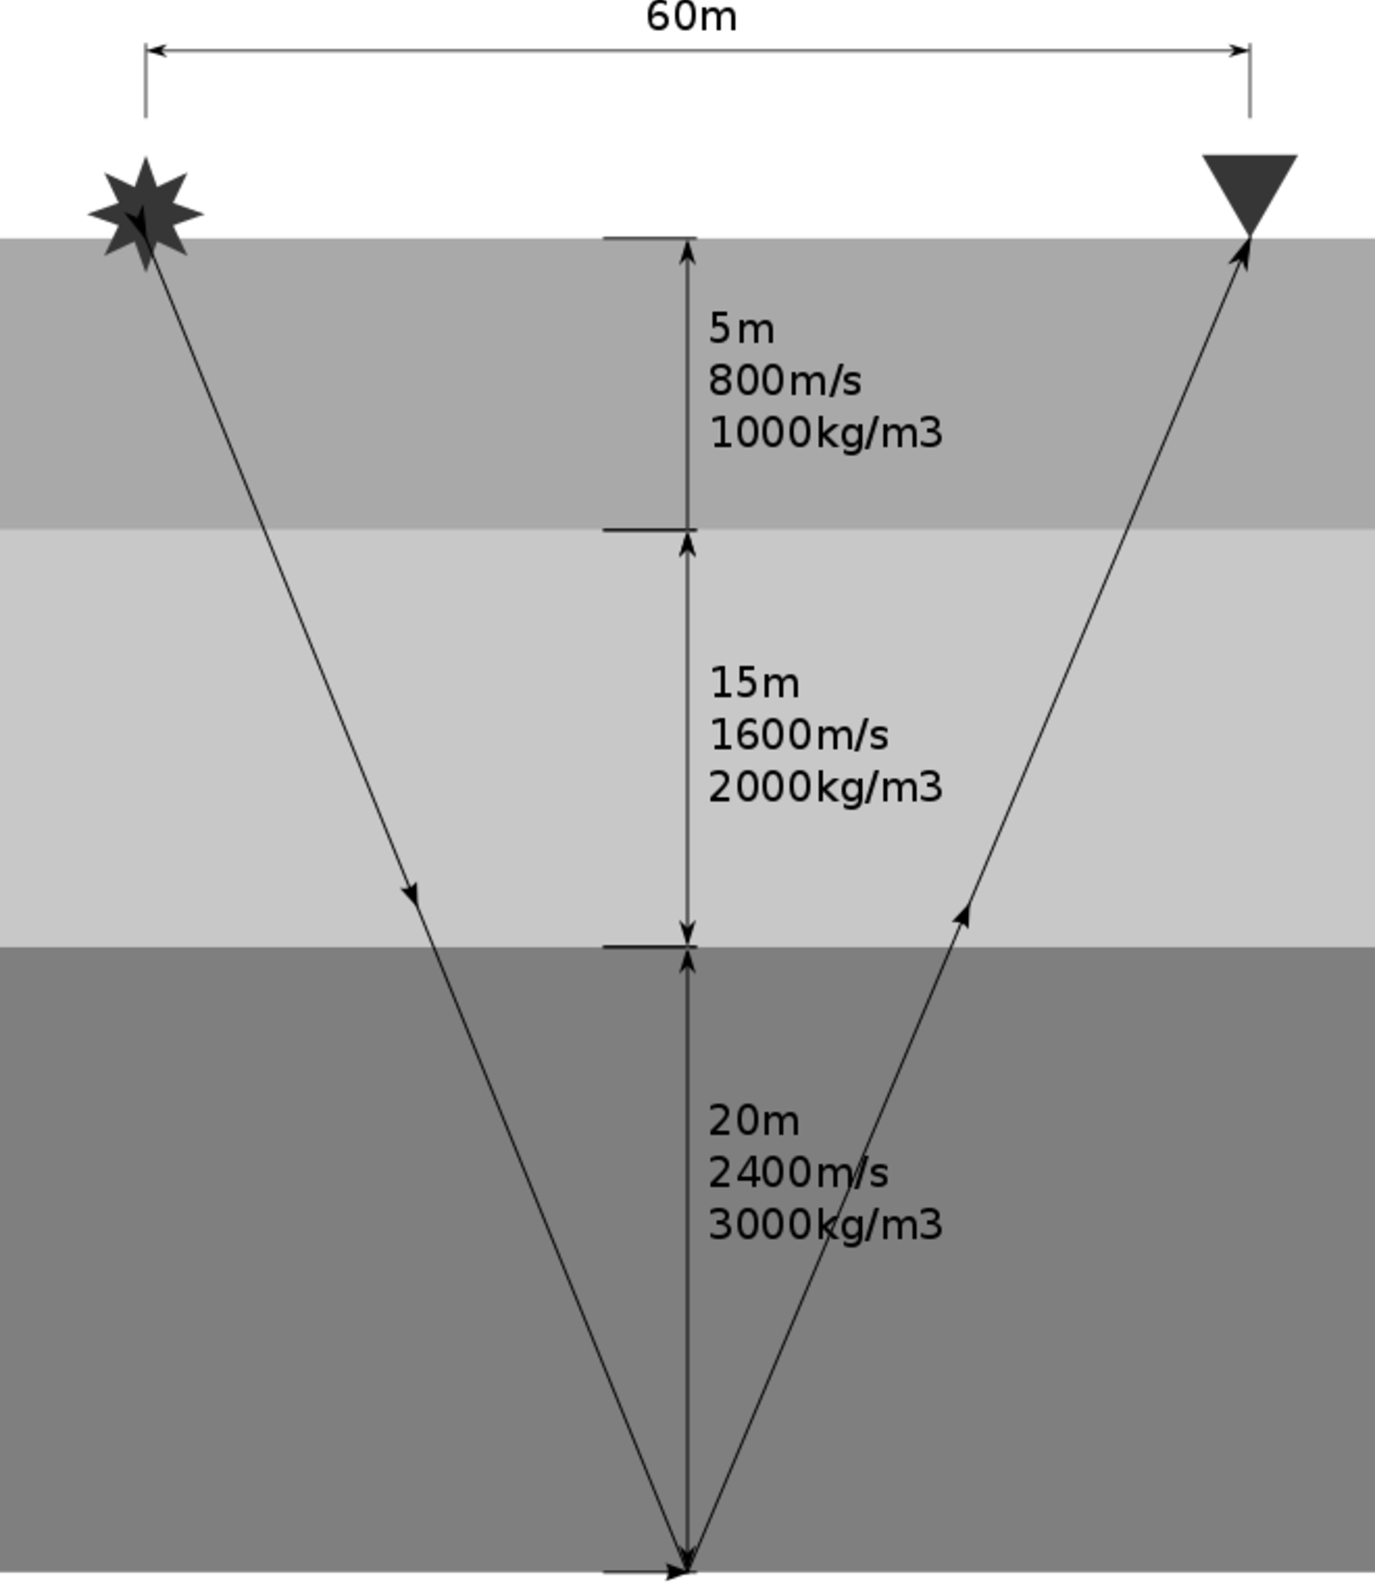
\includegraphics[width=0.8\textwidth]{model.pdf}
\caption{Seismic Model. The star is the source location and the triangle a geophone. This model assumes straight rays.}
\end{figure}
\newpage
\section*{Revision}
\section{The Convolutional Model}
\subsection{}
Describe in words what convolution is, and how it differs from correlation. Give an example of where you might use a) convolution and b) correlation.
\subsection{}
The convolutional model of the seismic trace states that the trace we record is the result of the earth's response convolved with the source wavelet and the recording system, with some additional noise. Show an equation which describes this, and label each term.
\subsection{}
The earth's response consists of a range of different signals, including the direct wave, refracted wave and reflected wave.  Modify the convolutional model equation to include these signals.
\section{The Direct Wave}
\subsection{}
What is the direct wave?
\subsection{}
Assuming a velocity of 400m/s, how long does it take the direct wave to travel from the source to receiver shown in Figure 1?
\subsection{}
Attenuation of waves occurs for a number of reasons. One reason is that of spherical divergence. Describe the basic cause of amplitude loss due to spherical divergence.
\subsection{}
Briefly discuss one other cause of wave attenuation in seismic data.
\subsection{}
Assuming that the attenuation due to spherical divergence has a coefficient of two, and the source has unit amplitude, calculate the amplitude of the direct wave at the geophone in Figure 1.
\section{The Refracted Wave}
\subsection{}
What is a refracted wave? What is one potential use of the refracted wave data?
\subsection{}
What is the critical angle at the bottom of the first layer in the source-receiver geometry shown in Figure 1?
\subsection{}
What is the travel time for the geometry shown in Figure 1?
\newpage
\section{The Reflected Wave}
\subsection{}
Calculate the travel time of the reflected wave for the model shown in Figure 1. Assume straight rays.
\subsection{}
Discuss how you would analytically calculate the correct (non-straight) ray path.
\subsection{}
Assuming a unit source amplitude, calculate the amplitude of the reflected wave at the geophone due to transmission and reflection coefficients.  Assume zero offset coefficients.
\par~\\
Discuss when it might and might not be appropriate to use the zero offset assumption.

\section{Seismic Gathers}
\subsection{}
What is the difference between a shot gather, a receiver gather and  CMP gather? Draw a rough diagram of each.  
\subsection{}
What are CMP gathers useful for? Why?
\subsection{}
What assumptions are made when CMP stacking? What happens when these assumptions break down?
\subsection{}
What is fold?
\section{Amplitude Recovery}
\subsection{}
Why is amplitude recovery used?
\subsection{}
Why is using an AGC for amplitude recovery not ideal?
\section{Normal Moveout}
\subsection{}
Draw a rough diagram showing why normal moveout is hyperbolic.
\subsection{}
Calculate the zero offset travel-time for the reflection event in question 4.
\subsection{}
Wavelet stretching is caused by the non-linear NMO correction. Discuss the impact of stretch and a potential mitigation strategy.
\section{Stacking}
\subsection{}
What is stacking?  
\subsection{}
What is the signal to noise ratio improvement for a CMP gather with a fold of $n$?
\section{Noise attenuation}
\subsection{}
The refracted wave calculated in question 3 is often considered noise.  What is one method that can be used to remove the refracted wave? Discuss the steps required in this method.
\subsection{}
Often we want to enhance coherent events whilst attenuating random events. Discuss one method for achieving this. Discuss the potential negatives associated with this method.
\section{Spectral Analysis}
Briefly discuss what a fourier transform does.  Draw a rough diagram of the spectral analysis of two sine waves that have been mixed together.  On the spectral diagram, draw a filter that could be used to separate the two signals.  Discuss how this might be useful for seismic data.  Discuss the spectral content of the 3 common seismic waves- ground roll, refractor and reflector.
\section{Processing Flows}
\subsection{}
Suggest a simple processing flow for a seismic dataset, using the processes discussed from question 5 to question 9.  State why you chose that particular processing sequence.  State any key parameters which need to be tested.

\newpage
\section{Useful Formulas}
\[R = \frac{1}{distance^2}\]
\[T = \frac{X}{V_1} + \frac{2z \cos{i_c}}{V_0}, \quad i_c = \sin^{-1}{\frac{V_0}{V_1}} \]
Where
\begin{itemize}
\item $X$ = lateral distance
\item $V_0$ = velocity of weathering layer
\item $V_1$ = velocity of sub-weathering layer
\item $z$ = thickness of weathering layer
\item $i_c$ = critical angle
\end{itemize}

\[ R_r = \frac{z_1 - z_0}{z_1+z_0}\]
\[ R_t = \frac{2*z_0}{z_1+z_0}\]
where 
\begin{itemize}
\item $z_0$  = acoustic contrast in layer 0, i.e. $\rho_0 v_0$
\item $z_1$ = acoustic contrast in layer 1, i.e. $\rho_1 v_1$
\end{itemize}

\[ {t_x}^2 = {t_0}^2 + \frac{x^2}{v^2}\]
where
\begin{itemize}
\item $t_x$ is the travel time at offset x
\item $t_0$ is the travel-time at offset 0
\item $x$ is the offset
\item $v$ is the velocity
\end{itemize}

\[ x_{rms} = \sqrt{\frac{1}{n}\left(x_1^2+x_2^2+\cdots+x_n^2\right)}\]

where
\begin{itemize}
\item $x_n$ is the sample number
\item $n$ is the number of samples
\end{itemize}

%\newpage
%\lstinputlisting{../exercise1.py}
%\lstinputlisting{../exercise2.py}
%\lstinputlisting{../exercise3.py}
%\lstinputlisting{../exercise4.py}
%\lstinputlisting{../exercise5.py}
%\lstinputlisting{../exercise6.py}
%\lstinputlisting{../exercise7.py}
%\lstinputlisting{../exercise8.py}
%\lstinputlisting{../exercise9.py}


\end{document}